\documentclass[]{article}
\usepackage{lmodern}
\usepackage{amssymb,amsmath}
\usepackage{ifxetex,ifluatex}
\usepackage{fixltx2e} % provides \textsubscript
\ifnum 0\ifxetex 1\fi\ifluatex 1\fi=0 % if pdftex
  \usepackage[T1]{fontenc}
  \usepackage[utf8]{inputenc}
\else % if luatex or xelatex
  \ifxetex
    \usepackage{mathspec}
  \else
    \usepackage{fontspec}
  \fi
  \defaultfontfeatures{Ligatures=TeX,Scale=MatchLowercase}
\fi
% use upquote if available, for straight quotes in verbatim environments
\IfFileExists{upquote.sty}{\usepackage{upquote}}{}
% use microtype if available
\IfFileExists{microtype.sty}{%
\usepackage[]{microtype}
\UseMicrotypeSet[protrusion]{basicmath} % disable protrusion for tt fonts
}{}
\PassOptionsToPackage{hyphens}{url} % url is loaded by hyperref
\usepackage[unicode=true]{hyperref}
\hypersetup{
            pdftitle={Project 2 -- Identifying and Addressing High Impact Natural Disasters},
            pdfauthor={Me, Dhruv Singh},
            pdfborder={0 0 0},
            breaklinks=true}
\urlstyle{same}  % don't use monospace font for urls
\usepackage[margin=1in]{geometry}
\usepackage{color}
\usepackage{fancyvrb}
\newcommand{\VerbBar}{|}
\newcommand{\VERB}{\Verb[commandchars=\\\{\}]}
\DefineVerbatimEnvironment{Highlighting}{Verbatim}{commandchars=\\\{\}}
% Add ',fontsize=\small' for more characters per line
\usepackage{framed}
\definecolor{shadecolor}{RGB}{248,248,248}
\newenvironment{Shaded}{\begin{snugshade}}{\end{snugshade}}
\newcommand{\KeywordTok}[1]{\textcolor[rgb]{0.13,0.29,0.53}{\textbf{#1}}}
\newcommand{\DataTypeTok}[1]{\textcolor[rgb]{0.13,0.29,0.53}{#1}}
\newcommand{\DecValTok}[1]{\textcolor[rgb]{0.00,0.00,0.81}{#1}}
\newcommand{\BaseNTok}[1]{\textcolor[rgb]{0.00,0.00,0.81}{#1}}
\newcommand{\FloatTok}[1]{\textcolor[rgb]{0.00,0.00,0.81}{#1}}
\newcommand{\ConstantTok}[1]{\textcolor[rgb]{0.00,0.00,0.00}{#1}}
\newcommand{\CharTok}[1]{\textcolor[rgb]{0.31,0.60,0.02}{#1}}
\newcommand{\SpecialCharTok}[1]{\textcolor[rgb]{0.00,0.00,0.00}{#1}}
\newcommand{\StringTok}[1]{\textcolor[rgb]{0.31,0.60,0.02}{#1}}
\newcommand{\VerbatimStringTok}[1]{\textcolor[rgb]{0.31,0.60,0.02}{#1}}
\newcommand{\SpecialStringTok}[1]{\textcolor[rgb]{0.31,0.60,0.02}{#1}}
\newcommand{\ImportTok}[1]{#1}
\newcommand{\CommentTok}[1]{\textcolor[rgb]{0.56,0.35,0.01}{\textit{#1}}}
\newcommand{\DocumentationTok}[1]{\textcolor[rgb]{0.56,0.35,0.01}{\textbf{\textit{#1}}}}
\newcommand{\AnnotationTok}[1]{\textcolor[rgb]{0.56,0.35,0.01}{\textbf{\textit{#1}}}}
\newcommand{\CommentVarTok}[1]{\textcolor[rgb]{0.56,0.35,0.01}{\textbf{\textit{#1}}}}
\newcommand{\OtherTok}[1]{\textcolor[rgb]{0.56,0.35,0.01}{#1}}
\newcommand{\FunctionTok}[1]{\textcolor[rgb]{0.00,0.00,0.00}{#1}}
\newcommand{\VariableTok}[1]{\textcolor[rgb]{0.00,0.00,0.00}{#1}}
\newcommand{\ControlFlowTok}[1]{\textcolor[rgb]{0.13,0.29,0.53}{\textbf{#1}}}
\newcommand{\OperatorTok}[1]{\textcolor[rgb]{0.81,0.36,0.00}{\textbf{#1}}}
\newcommand{\BuiltInTok}[1]{#1}
\newcommand{\ExtensionTok}[1]{#1}
\newcommand{\PreprocessorTok}[1]{\textcolor[rgb]{0.56,0.35,0.01}{\textit{#1}}}
\newcommand{\AttributeTok}[1]{\textcolor[rgb]{0.77,0.63,0.00}{#1}}
\newcommand{\RegionMarkerTok}[1]{#1}
\newcommand{\InformationTok}[1]{\textcolor[rgb]{0.56,0.35,0.01}{\textbf{\textit{#1}}}}
\newcommand{\WarningTok}[1]{\textcolor[rgb]{0.56,0.35,0.01}{\textbf{\textit{#1}}}}
\newcommand{\AlertTok}[1]{\textcolor[rgb]{0.94,0.16,0.16}{#1}}
\newcommand{\ErrorTok}[1]{\textcolor[rgb]{0.64,0.00,0.00}{\textbf{#1}}}
\newcommand{\NormalTok}[1]{#1}
\usepackage{graphicx,grffile}
\makeatletter
\def\maxwidth{\ifdim\Gin@nat@width>\linewidth\linewidth\else\Gin@nat@width\fi}
\def\maxheight{\ifdim\Gin@nat@height>\textheight\textheight\else\Gin@nat@height\fi}
\makeatother
% Scale images if necessary, so that they will not overflow the page
% margins by default, and it is still possible to overwrite the defaults
% using explicit options in \includegraphics[width, height, ...]{}
\setkeys{Gin}{width=\maxwidth,height=\maxheight,keepaspectratio}
\IfFileExists{parskip.sty}{%
\usepackage{parskip}
}{% else
\setlength{\parindent}{0pt}
\setlength{\parskip}{6pt plus 2pt minus 1pt}
}
\setlength{\emergencystretch}{3em}  % prevent overfull lines
\providecommand{\tightlist}{%
  \setlength{\itemsep}{0pt}\setlength{\parskip}{0pt}}
\setcounter{secnumdepth}{0}
% Redefines (sub)paragraphs to behave more like sections
\ifx\paragraph\undefined\else
\let\oldparagraph\paragraph
\renewcommand{\paragraph}[1]{\oldparagraph{#1}\mbox{}}
\fi
\ifx\subparagraph\undefined\else
\let\oldsubparagraph\subparagraph
\renewcommand{\subparagraph}[1]{\oldsubparagraph{#1}\mbox{}}
\fi

% set default figure placement to htbp
\makeatletter
\def\fps@figure{htbp}
\makeatother


\title{Project 2 -- Identifying and Addressing High Impact Natural Disasters}
\author{Me, Dhruv Singh}
\date{December 24, 2019}

\begin{document}
\maketitle

Synopsis:

This project utilizes years of data on storm tracking starting from
1950s onwards in order to answer the question - Which natural disasters
are most disasterous to human life and economic activity?

In order to do so, it treats fatalities and injuries as indicators of
damage to human life. Tabulating by the type of disaster, we are able to
obtain an estimate of the types of disasters that have the highest
impact on human life, and to safeguard against it accordingly.

\subsection{PART 0: SETUP}\label{part-0-setup}

echo settings for embedding code

Setting Directory

\begin{Shaded}
\begin{Highlighting}[]
\KeywordTok{getwd}\NormalTok{()}
\end{Highlighting}
\end{Shaded}

\begin{verbatim}
## [1] "C:/Dhruv/misc/data/R_5_reproducible_research/wk4_documenting"
\end{verbatim}

\begin{Shaded}
\begin{Highlighting}[]
\KeywordTok{setwd}\NormalTok{(}\StringTok{"C:/Dhruv/misc/data/R_5_reproducible_research/wk4_documenting"}\NormalTok{)}
\end{Highlighting}
\end{Shaded}

\subsection{PART I: PREPROCESSING DATA}\label{part-i-preprocessing-data}

Reading in strom data csv bz2:

\begin{Shaded}
\begin{Highlighting}[]
\NormalTok{storm_data <-}\StringTok{ }\KeywordTok{read.csv}\NormalTok{(}\StringTok{"repdata_data_StormData.csv.bz2"}\NormalTok{)}
\end{Highlighting}
\end{Shaded}

Loading up necessary packages:

\begin{Shaded}
\begin{Highlighting}[]
\CommentTok{# install.packages("knitr", repos='http://cran.us.r-project.org')}
\CommentTok{# install.packages("rsconnect", repos='http://cran.us.r-project.org')}
\KeywordTok{library}\NormalTok{(knitr)}
\KeywordTok{library}\NormalTok{(ggplot2)}
\KeywordTok{library}\NormalTok{(rsconnect)}
\end{Highlighting}
\end{Shaded}

\begin{verbatim}
## Warning: package 'rsconnect' was built under R version 3.6.2
\end{verbatim}

Converting data type for categorical analysis:

\begin{Shaded}
\begin{Highlighting}[]
\NormalTok{storm_data}\OperatorTok{$}\NormalTok{EVTYPE <-}\StringTok{ }\KeywordTok{as.character}\NormalTok{(storm_data}\OperatorTok{$}\NormalTok{EVTYPE)}
\end{Highlighting}
\end{Shaded}

Aggregating data to produce summary plots:

\begin{Shaded}
\begin{Highlighting}[]
\NormalTok{storm_agg <-}\StringTok{ }\KeywordTok{aggregate}\NormalTok{(FATALITIES }\OperatorTok{~}\StringTok{ }\NormalTok{EVTYPE, storm_data, }\DataTypeTok{FUN =}\NormalTok{ sum)}
\CommentTok{# subsetting to only the highest damage incidents}
\NormalTok{storm_agg <-}\StringTok{ }\NormalTok{storm_agg[storm_agg}\OperatorTok{$}\NormalTok{FATALITIES }\OperatorTok{>}\StringTok{ }\DecValTok{100}\NormalTok{ ,]}

\CommentTok{# doing the same for property damage as economic loss indicator}
\NormalTok{storm_agg2 <-}\StringTok{ }\KeywordTok{aggregate}\NormalTok{(PROPDMG }\OperatorTok{~}\StringTok{ }\NormalTok{EVTYPE, storm_data, }\DataTypeTok{FUN =}\NormalTok{ sum)}
\CommentTok{# subsetting to only the highest damage incidents}
\NormalTok{storm_agg2 <-}\StringTok{ }\NormalTok{storm_agg2[storm_agg2}\OperatorTok{$}\NormalTok{PROPDMG }\OperatorTok{>}\StringTok{ }\DecValTok{26000}\NormalTok{ ,]}
\end{Highlighting}
\end{Shaded}

\subsection{PART II: RESULTS}\label{part-ii-results}

Relevant plots for human damage:

\begin{Shaded}
\begin{Highlighting}[]
\CommentTok{# building plot}
\NormalTok{highest_mortality <-}\StringTok{ }\KeywordTok{ggplot}\NormalTok{(storm_agg, }\KeywordTok{aes}\NormalTok{(}\DataTypeTok{x =}\NormalTok{ storm_agg}\OperatorTok{$}\NormalTok{EVTYPE, }\DataTypeTok{y =}\NormalTok{ storm_agg}\OperatorTok{$}\NormalTok{FATALITIES)) }\OperatorTok{+}\StringTok{ }
\StringTok{  }\KeywordTok{geom_bar}\NormalTok{(}\DataTypeTok{stat =} \StringTok{"identity"}\NormalTok{, }\DataTypeTok{fill =} \StringTok{"steelblue"}\NormalTok{) }\OperatorTok{+}\StringTok{ }\KeywordTok{labs}\NormalTok{(}\DataTypeTok{x =} \StringTok{"Event Type"}\NormalTok{, }\DataTypeTok{y =} \StringTok{"Fatalities"}\NormalTok{, }\DataTypeTok{title =} \StringTok{"Fatalities by Event Type"}\NormalTok{) }\OperatorTok{+}\StringTok{ }
\StringTok{  }\KeywordTok{theme}\NormalTok{(}\DataTypeTok{axis.text.x =} \KeywordTok{element_text}\NormalTok{(}\DataTypeTok{angle =} \DecValTok{90}\NormalTok{), }\DataTypeTok{legend.position=}\StringTok{"none"}\NormalTok{)}

\CommentTok{# printing plot}
\NormalTok{highest_mortality}
\end{Highlighting}
\end{Shaded}

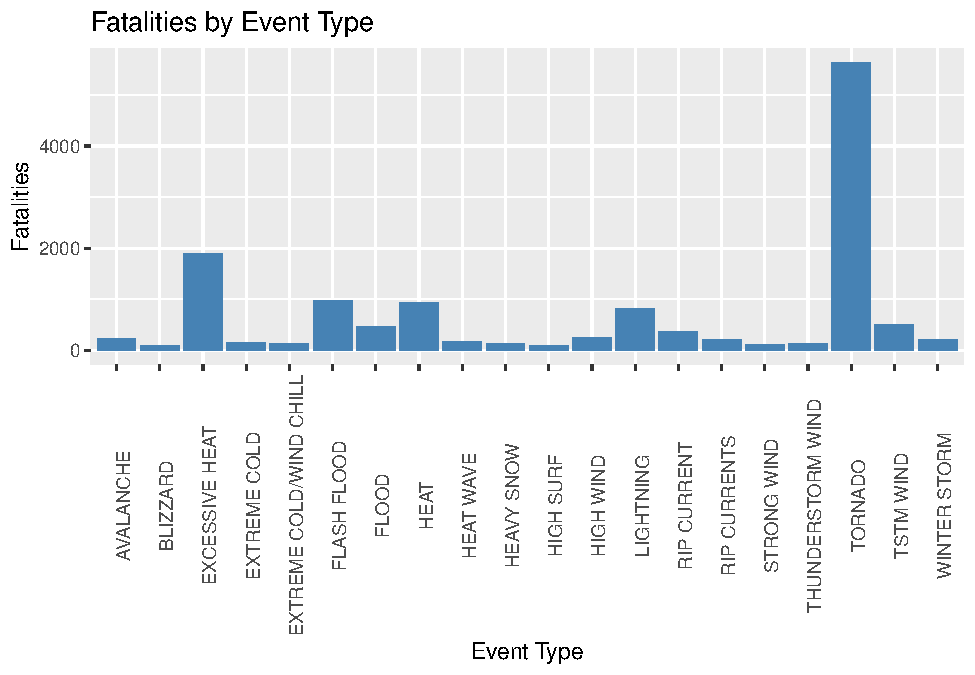
\includegraphics{Project2_files/figure-latex/plots-1.pdf}

In the results we find that the most damaging natural disasters include
Tornados and Excessive Heat, followed by Flash Floods and Lightening.
All of which contain an element of unpredictability, but can be foreseen
when regular inclement weather takes on more menacing features. And
should therefore be safeguarded against.

Relevant plots for property damage:

\begin{Shaded}
\begin{Highlighting}[]
\CommentTok{# building plot}
\NormalTok{highest_prop.loss <-}\StringTok{ }\KeywordTok{ggplot}\NormalTok{(storm_agg2, }\KeywordTok{aes}\NormalTok{(}\DataTypeTok{x =}\NormalTok{ storm_agg2}\OperatorTok{$}\NormalTok{EVTYPE, }\DataTypeTok{y =}\NormalTok{ storm_agg2}\OperatorTok{$}\NormalTok{PROPDMG)) }\OperatorTok{+}\StringTok{ }
\StringTok{  }\KeywordTok{geom_bar}\NormalTok{(}\DataTypeTok{stat =} \StringTok{"identity"}\NormalTok{, }\DataTypeTok{fill =} \StringTok{"steelblue"}\NormalTok{) }\OperatorTok{+}\StringTok{ }\KeywordTok{labs}\NormalTok{(}\DataTypeTok{x =} \StringTok{"Event Type"}\NormalTok{, }\DataTypeTok{y =} \StringTok{"Property Damage"}\NormalTok{, }\DataTypeTok{title =} \StringTok{"Property Damage by Event Type"}\NormalTok{) }\OperatorTok{+}\StringTok{ }
\StringTok{  }\KeywordTok{theme}\NormalTok{(}\DataTypeTok{axis.text.x =} \KeywordTok{element_text}\NormalTok{(}\DataTypeTok{angle =} \DecValTok{90}\NormalTok{), }\DataTypeTok{legend.position=}\StringTok{"none"}\NormalTok{)}

\CommentTok{# printing plot}
\NormalTok{highest_prop.loss}
\end{Highlighting}
\end{Shaded}

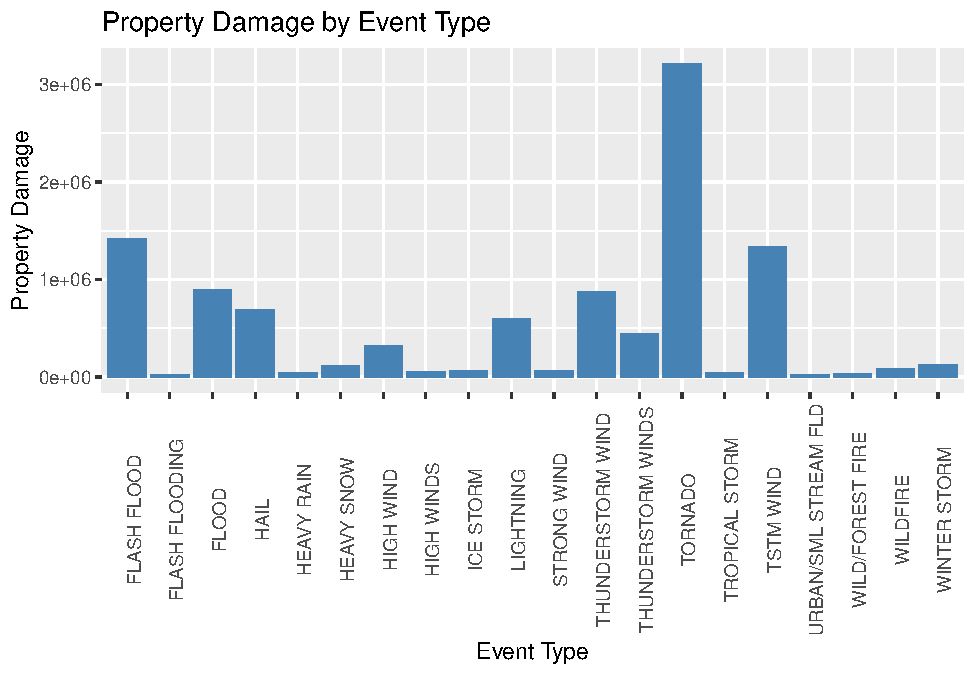
\includegraphics{Project2_files/figure-latex/plots econ-1.pdf}

Once again, we find that Tornados and Flash Floods cause the greatest
damage to property, followed by what is abbreviated as TSTM Wonds!

Relevant tables:

\begin{Shaded}
\begin{Highlighting}[]
\CommentTok{# producing table of overall stats}
\KeywordTok{summary}\NormalTok{(storm_data}\OperatorTok{$}\NormalTok{FATALITIES)}
\end{Highlighting}
\end{Shaded}

\begin{verbatim}
##     Min.  1st Qu.   Median     Mean  3rd Qu.     Max. 
##   0.0000   0.0000   0.0000   0.0168   0.0000 583.0000
\end{verbatim}

\begin{Shaded}
\begin{Highlighting}[]
\CommentTok{# tabulating damage stats}
\KeywordTok{summary}\NormalTok{(storm_data}\OperatorTok{$}\NormalTok{PROPDMG)}
\end{Highlighting}
\end{Shaded}

\begin{verbatim}
##    Min. 1st Qu.  Median    Mean 3rd Qu.    Max. 
##    0.00    0.00    0.00   12.06    0.50 5000.00
\end{verbatim}

\section{fatalities stats}\label{fatalities-stats}

Min. 1st Qu. Median Mean 3rd Qu. Max. 0.0000 0.0000 0.0000 0.0168 0.0000
583.0000

\section{property damage stats}\label{property-damage-stats}

Min. 1st Qu. Median Mean 3rd Qu. Max. 0.00 0.00 0.00 12.06 0.50 5000.00

\begin{Shaded}
\begin{Highlighting}[]
\CommentTok{# knit("C:/Dhruv/misc/data/R_5_reproducible_research/wk4_documenting/Project2.Rmd",output="C:/Dhruv/misc/data/R_5_reproducible_research/wk4_documenting/Project2.html")}
\end{Highlighting}
\end{Shaded}

\end{document}
